\documentclass[a4paper,oneside, 12pt]{article}
\usepackage[margin=0.7in]{geometry}

\usepackage[cm-default]{fontspec}
\usepackage{xunicode}
\usepackage{xltxtra}

\usepackage{xgreek}

\setmainfont[Mapping=tex-text]{Linux Libertine O}
\usepackage{graphicx}
\usepackage{fancyvrb}
\usepackage{listings}
\usepackage{xcolor}
\usepackage[section]{placeins}


\title{
	\textbf{Κατανεμημένα Συστήματα}\\
	\textbf{Εξαμηνιαία Εργασία}\\
	Noobcash
 }
\author{
	Λαμπρινίδης-Λέντελ Βλαντισλάβ, 03114054
	\and
	Μαρμάνης Ιάσων, 03114088
	\and
	Μαυρομμάτης Ιάσων, 03114771
}
\lstset{basicstyle=\ttfamily,
	showstringspaces=false,
	commentstyle=\color{red},
	keywordstyle=\color{blue}
}

\date{\today}

\begin{document}
	
\maketitle

\section{Σκοπός}
Στην εργασία αυτή υλοποιήσαμε ένα κατανεμημένο σύστημα που υλοποιεί την τεχνολογία του 
blockchain.
Η εφαρμογή αποτελείται από ένα backend που μιλάει με τα τους άλλους κόμβους, και ένα cli tool που δέχεται εντολές από τον χρήστη και τις προωθεί στο backend.

\section{Αρχιτεκτονική}
\subsection{Επικοινωνία}
Κάθε backend πρέπει να έχει ένα duplex δίαυλο επικοινωνίας με κάθε άλλο κόμβο (peer) και με το cli.
Η επικοινωνία αυτή γίνεται μέσω TCP sockets. Για κάθε peer υπάρχουν 2 threads, ένα που διαχειρίζεται τα εισερχόμενα μηνύματα και ένα τα εξερχόμενα. 

Η επικοινωνία με το main thread γίνεται με message-passing : τα εισερχόμενα μηνύματα μπαίνουν σε μία blocking queue από την οποία διαβάζει συνεχώς το main thread. Όμοια διαχειριζόμαστε τα εξερχόμενα μηνύματα. Η επιλογή να γίνεται όλη η επεξεργασία από το main thread έγινε επειδή για κάθε εισερχόμενο αίτημα θα χρειαζόταν ούτως η άλλως πρόσβαση σε global δομές, άρα θα έπρεπε να τις κλειδώσει και έτσι πάλι η επεξεργασία θα γινόταν σειριακά. Επίσης υπάρχει ένα thread για την επικοινωνία (duplex) με το cli και ένα thread για τον miner. Πάλι η επικοινωνία γίνεται με message passing.

\subsection{Blockchain}
\subsubsection{Δομές}
Κάθε κόμβος διατηρεί τις εξής δομές:

\begin{itemize}
	\item Transaction pool
	\item Blockchain
	\item Confirmed UTXOs
	\item Unconfirmed UTXOs
\end{itemize}

\subsubsection{Ορισμοί και αναλλοίωτες}
Confirmed transactions ονομάζουμε τις συναλλαγές που είναι σε block που έχουμε στο chain μας.
To confirmed UTXO set είναι το set που θα δει κάποιος αν εφαρμόσει ένα-ένα τα confirmed transactions στο set που περιέχει μόνο το genesisTransactionOutput. 

Στο transaction pool βρίσκονται όλα τα transactions τα οποία έχουν γίνει validated αλλά δεν έχουν μπει στο chain. Για το validation τους χρησιμοποιείται το unconfirmed UTXO set που εν τέλει είναι το set που θα δει κανείς αν εφαρμόσει τα transations του Transaction Pool στο confirmed UTXO set.

Τα αιτήματα για το balance ενός peer και για την δημιουργία-επαλήθευση μίας συναλλαγής εξυπηρετούνται με βάση το unconfirmed UTXO set.

Ένα transaction είναι valid με βάση ένα UTXO set αν
\begin{itemize}
	\item Έχει έγκυρη υπογραφή
	\item Έχει έγκυρο txid (hash των δεδομένων του)
	\item Όλα τα inputs του αντιστοιχούν σε υπάρχοντα outputs στο UTXOs
	\item Τα προαναφερθέντα outputs ανήκουν πράγματι στον αποστολέα
	\item Το άθροισμα των τιμών που αντιστοιχούν στα inputs ισούται με το άθροισμα των
	τιμών που αντιστοιχούν  στα outputs
\end{itemize}

Ένα block είναι valid με βάση ένα chain  και το αντίστοιχο confirmed UTXO set αν
\begin{itemize}
	\item Έχει έγκυρη δομή : σωστό PoW (nonce) - hash
	\item Έχει σωστό previous hash και index (το αναμενόμενο με βάση το τελευταίο block του chain)
	\item Είναι έγκυρη η εφαρμογή των transactions του ένα προς ένα πάνω στο confiremd UTXO set
\end{itemize}

\subsubsection{Σενάρια χρήσης}
\paragraph{Cli transaction request}
Με την λήψη ενός αιτήματος για νέα συναλλαγή από το cli, το backend ελέγχει αν ο κόμβος έχει αρκετά coins, και αν έχει τότε το δημιουργεί, το εφαρμόζει στο unconfirmed UTXO set, το προσθέτει στο transaction pool και το κάνει broadcast.

\paragraph{New transaction}
Κατά την λήψη μίας νέας συναλλαγής από ένα κόμβο, ελέγχεται η εγκυρότητα της με βάση το unconfirmed UTXO set στο οποίο και προστίθεται αν είναι έγκυρη. Επίσης τότε προστίθεται και στο transaction pool.

\paragraph{New block}
Κατά την λήψη ενός block ελέγχεται η εγκυρότητα του με βάση το chain και το confirmed UTXO set.
Αν είναι έγκυρο, τότε εφαρμόζονται τα νέα transactions και προκύπτει το νέο confirmed UTXO set.
Ύστερα αφαιρούνται από το transaction pool τα transaction που υπήρχαν στο νέο block.
Τέλος δημιουργείται εκ νέου το νέο unconfirmed UTXO set με την εφαρμογή των εναπομεινάντων συναλλαγών του transaction pool στο confirmed UTXO set. Μερικές από αυτές μπορεί πλέον να μην είναι έγκυρες και έτσι αφαιρούνται.
Αν το block έχει έγκυρη δομή αλλά έχει μεγαλύτερο index από το αναμενόμενο τότε ζητείται από τον αποστολέα η αλυσίδα του για να γίνει αντικατάσταση σε περίπτωση που είναι μεγαλύτερη.

\paragraph{Concensus - new chain}
Κατά την λήψη μία νέας αλυσίδας, που γίνεται μετά από αίτημα του κόμβου, ελέγχεται αρχικά ότι η αλυσίδα είναι μεγαλύτερη από την υπάρχουσα. Σε περίπτωση που είναι, ελέγχεται η εγκυρότητα των blocks ξεκινώντας από το genesis block και ένα confirmed UTXO set που περιέχει μόνο το genesis Transaction Output. Αν είναι, τότε η αλυσίδα γίνεται δεκτή, το confirmed UTXO set αντικαθίσταται με αυτό που μόλις δημιουργήθηκε, όλες οι συναλλαγές του νέου chain αφαιρούνται από το transaction pool και δημιουργείται κατά τα γνωστά το νέο unconfirmed UTXO set.

\paragraph{Mining}
Κάθε αίτημα που οδηγεί σε αλλαγή του transaction pool ή του τελευταίου block οδηγεί σε απόπειρα έναρξης του mining. Συγκεκριμένα, αν το transaction pool έχει αρκετά transactions, δημιουργείται ένα νέο block με βάση το τελευταίο της αλυσίδας και αποστέλλεται στον miner. Αν χρειάζεται, διακόπτεται πιθανό mining που είναι ήδη σε εξέλιξη. Όταν το mining τελειώσει (αν γίνει αυτό, αφού μπορεί να διακοπεί) το νέο block στέλνεται πίσω στο main thread. Η διαχείριση του νέου block γίνεται όπως θα γινόταν αν το block ερχόταν από έναν άλλο κόμβο, αλλά σε περίπτωση που προστεθεί στην αλυσίδα γίνεται και broadcast στους υπόλοιπους κόμβους.

\subsection{Εργαλεία}
Η έναρξη του noobcash backend γίνεται μέσω του nbcd scirpt που δέχεται τις εξής παραμέτρους:
\begin{itemize}
	\item -n : πλήθος κόμβων
	\item -c : μέγεθος του block
	\item -d : δυσκολία του PoW
	\item -p : πόρτα για επικοινωνία, προαιρετική (default = 5000).
	\item -b : bootstrap node flag (αν τεθεί τότε port = 5000)
\end{itemize}

Η έναρξη του cli γίνεται μέσω του cli script που δέχεται τις εξής παραμέτρους:
\begin{itemize}
	\item -p : πόρτα που χρησιμοποιεί το αντίστοιχο backend, προαιρετική (default = 5000)
	\item -f : διάβασμα και αποστολή των transaction που υπάρχουν στο αντίστοιχο αρχείο κατά την έναρξη, προαιρετικό
	\item -t : χρήση των transaction files κάτω από τον φάκελο 10nodes, αντί για του 5nodes, προαιρετικό
\end{itemize}

Και τα δύο scripts είναι απλά wrappers που καλούν το gradlew με τις παραμέτρους που δίνονται.

Η IP διεύθυνση του bootstrap είναι hardcoded σε αυτή που χρησιμοποιήθηκε κατά την διεξαγωγή των πειραμάτων (192.168.0.1, private network). Πολύ εύκολα μπορεί να αλλάξει, αλλάζοντας μία γραμμή του κώδικα (Backend.java).
\section{Μετρήσεις}
Για διάφορες τιμές του πλήθους κόμβων, μεγέθους block και δυσκολίας PoW, σηκώσαμε τα backends και εκτελέσαμε για κάθε κόμβο, την ίδια στιγμή, το σενάριο που μας δόθηκε : διάβασμα αντίστοιχου αρχείου και αποστολή αιτημάτων για συναλλαγές.

Το καλύτερο που μπορέσαμε να κάνουμε ήταν να βάλουμε το cli να εκτελείται με το -f flag σε συγκεκριμένη στιγμή:
\begin{lstlisting}[language=bash]
echo \"./cli -f\" | at 17:42
\end{lstlisting}

Αναλύσαμε τα log files που δημιούργησαν τα backends και παρουσιάζουμε σε γραφικές παραστάσεις τα αποτελέσματα.

Το block time υπολογίστηκε ως ο μέσος χρόνος που χρειάζεται για να γίνει mine ένα block και όχι ο μέσος χρόνος που χρειάζεται για να αυξηθεί το μήκος της αλυσίδας κατά ένα.


Το throughput υπολογίστηκε με βάση το σύνολο των transactions που ζητήθηκαν, όχι μόνο όσων υπήρχαν στην τελική αλυσίδα.


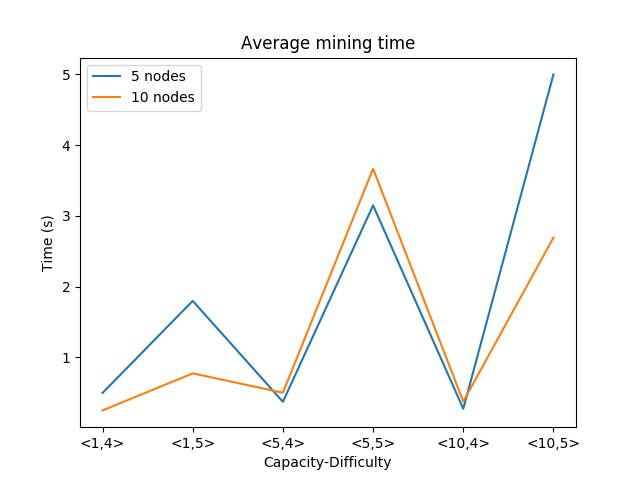
\includegraphics{avg_mine_time}

\paragraph{}
Για difficulty = 5 παρατηρούμε πως το average mining time αυξάνεται με την αύξηση του capacity, πιθανώς λόγω της υπολογιστικής επιβάρυνσης των μηχανημάτων. Σε ότι αφορά το scalability βλέπουμε πως με αύξηση των κόμβων, μόνο για ένα συνδυασμό $c,d = 5,5$ ο χρόνος αυξάνεται, σε κάθε άλλη περίπτωση μειώνεται. Από τη μία οι περισσότεροι κόμβοι επιβαρύνουν το δίκτυο, από την άλλη υπάρχει μεγαλύτερη πιθανότητα εύρεσης σωστού nonce (οι δοκιμές γίνονται τυχαία).

Επίσης το difficulty επηρεάζει και αυτό την μετρική με τον προφανή τρόπο.

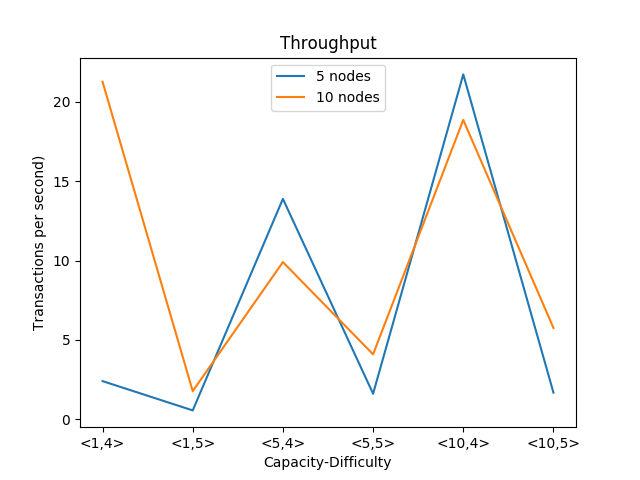
\includegraphics{tput}

Παρατηρούμε πως το throughput αυξάνεται με την αύξηση του capacity, αφού έτσι έχουμε λιγότερα μηνύματα στο δίκτυο. Για μεγαλύτερο difficulty το δίκτυο κάνει scale, ενώ με το μικρότερο όχι.

Το μεγάλο throughput στον συνδυασμό $c,d = 1,4$ ίσως είναι εικονικό αφού για τόσο συχνά blocks πολλά unconfirmed transactions καταλήγουν να γίνουν invalid, κάνοντας έτσι drop και πολλά άλλα transactions από το transaction pool.

\paragraph{}
Γενικά το σενάριο δεν είναι πολύ ρεαλιστικό και οι μετρήσεις αυτές ίσως να μην έχουν ιδιαίτερη αξία.
Θα έπρεπε να υπήρχαν πολύ περισσότεροι κόμβοι που κάνουν πιο σπάνια transactions (σε τυχαίους χρόνο), τα blocks να ήταν μεγαλύτερα όπως και το PoW difficulty. 

Στο σενάριο που εκτελέσαμε οι clients έστελναν περίπου 100 transactions όσο πιο γρήγορα μπορούσαν, χωρίς να περιμένουν καμία επιβεβαίωση. Αν ένα από αυτά αρχικά γινόταν accept αλλά μετά γινόταν dropped τότε θα μπορούσαν να καταλήξουν σχεδόν όλα ως invalid.

\paragraph{}


\end{document}